\documentclass[a4paper,12pt]{article}

% Language and input encoding
\usepackage[utf8]{inputenc}
\usepackage[spanish]{babel}

% Math packages
\usepackage{amsmath, amssymb, amsthm}

% Graphics and hyperlinks
\usepackage{graphicx}
\usepackage{hyperref}

% Page layout
\usepackage{geometry}
\geometry{margin=1in}

% Custom commands
\newtheorem{definition}{Definición}[section]
\newtheorem{theorem}{Teorema}[section]
\newtheorem{lemma}{Lema}[section]
\newtheorem{proposition}{Proposición}[section]

\title{\textbf{Demostraciones de NP-Completitud en Problemas}} 
\author{Daniel Machado Pérez \\
Diseño y Análisis de Algoritmos}
\date{}
\begin{document}

\maketitle
\tableofcontents
\newpage

\section*{Base Teórica .Problemas NP-Completos}

\begin{itemize}
    \item SAT
    \item 3-SAT
    \item k-Clique
    \item Conjunto Independiente
    \item Vertex Cover
    \item Subset Sum
    \item Mochila
    \item Hamilton (Dirigido)
    \item Viajante
\end{itemize}

\section{Exact Cover}


El problema \textbf{Exact Cover} puede describirse formalmente como sigue: 

\textbf{Entrada:} Un conjunto finito $X$ y una colección $S$ de subconjuntos de $X$.  \\
\textbf{Pregunta:} ¿Existe un subcolector $S' \subseteq S$ tal que cada elemento de $X$ aparezca \textbf{exactamente una vez} en los subconjuntos de $S'$?

\subsection{Pertenencia a NP}
Para demostrar que \textbf{Exact Cover} pertenece a la clase NP, debemos mostrar que, dada una solución candidata $S'$, es posible verificar en tiempo polinomial si $S'$ constituye una solución válida.

Dado que $|X| = n$ y $|S| = m$, la verificación puede realizarse de la siguiente manera:
\begin{enumerate}
    \item Crear un registro inicializado en cero para cada elemento $x \in X$.
    \item Para cada subconjunto $S_i \in S'$, incrementar el contador asociado a cada elemento $x \in S_i$.
    \item Comprobar que el contador de cada elemento en $X$ es exactamente igual a uno. Si esta condición se cumple, entonces $S'$ es una solución válida.
\end{enumerate}

\textbf{Conclusión:} Como la verificación puede completarse en tiempo polinomial respecto al tamaño de la entrada, \textbf{Exact Cover} pertenece a NP.

\subsection{NP-Hardness}
Demostraremos que \textbf{Exact Cover} es NP-Hard mediante una reducción desde \textbf{3-SAT} en tiempo polinomial 

\subsubsection{Demostración. Reducción desde 3-SAT}
Dada una fórmula booleana $F$ en forma normal conjuntiva con $n$ variables $x_1, x_2, \dots, x_n$ y $m$ cláusulas $C_1, C_2, \dots, C_m$, donde cada cláusula $C_i$ está formada por $l_i$ literales $L_{ik}$, construiremos una instancia del problema \textbf{Exact Cover} como sigue:
\begin{enumerate}
    \item Definimos el universo $U$ como:
    \[
    U = \{x_1, x_2, \dots, x_n\} \cup \{C_1, C_2, \dots, C_m\} \cup \{p_{ik} \mid C_i \text{ contiene el literal } L_{ik}\}.
    \]
    \item Construimos los subconjuntos $S$ de $U$ de la siguiente manera:
    \begin{itemize}
        \item Para cada literal $p_{ik}$, agregamos un subconjunto $S_{p_{ik}} = \{p_{ik}\}$.
        \item Para cada variable $x_j$:
        \begin{itemize}
            \item Si $x_j$ es \textit{True (T)} agregamos $S_{x_j,T}$, que contiene $x_j$ y todas sus instancias negativas.
            \item Si $x_j$ es \textit{False {F}} agregamos $S_{x_j,F}$, que contiene $x_j$ y todas sus instancias positivas.
        \end{itemize}
        \item Para cada cláusula $C_i$, agregamos subconjuntos $S_{C_{ik}} = \{C_i, p_{ik}\}$ para cada literal en $C_i$.
    \end{itemize}
\end{enumerate}

\textbf{Probemos que: Si $F$ es satisfacible, entonces la instancia de \textbf{Exact Cover} es \textit{True}.}

Sea $t$ una asignación de verdad que satisface $F$:
\begin{itemize}
    \item Para cada variable $x_j$, seleccionamos $S_{x_j,T}$ si $t(x_j) = \text{\textit{True}}$, o $S_{x_j,F}$ si $t(x_j) = \text{\textit{False}}$.
    \item Para cada cláusula $C_i$, seleccionamos un subconjunto $S_{C_{ik}}$ asociado a un literal $L_{ik}$ que sea verdadero en la asignación satisfactoria.
    \item Para terminar, para cada literal $p_{ik}$ que no haya sido cubierto, seleccionamos $S_{p_{ik}}$.
\end{itemize}
Esto cubre exactamente todos los elementos en $U$ $\Rightarrow$ cumple \textbf{Exact Cover}.

\textbf{Probemos que: Si la instancia de \textbf{Exact Cover} tiene solución, entonces $F$ es satisfacible.}
Sea $C$ una solución de \textbf{Exact Cover}:
\begin{itemize}
    \item Para cada variable $x_j$, el subconjunto seleccionado en $C$ determina si $x_j = \text{\textit{True}}$ o $x_j = \text{\textit{False}}$.
    \item Para cada cláusula $C_i$, existe un conjunto $S_{C_{jk}}$ en $C$ que cubre $C_i$. Por lo tanto, al menos uno de sus literales debe ser verdadero. Entonces, al menos un literal de cada cláusula debe ser verdadero.
\end{itemize}
Por lo tanto, la asignación correspondiente satisface $F$.

\subsubsection{Conclusión:} Dado que $F$ es satisfacible si y solo si la instancia de \textbf{Exact Cover} tiene solución, y la reducción se realiza en tiempo polinomial, \textbf{Exact Cover} es NP-Hard.

\subsection{NP-Completitud}
Dado que \textbf{Exact Cover} pertenece a NP y es NP-Hard, concluimos que es NP-Completo.





\section{3-Coloreo}

El problema \textbf{3-Coloreo} puede describirse formalmente de la siguiente manera:

\textbf{Entrada:} Un grafo no dirigido $G = (V, E)$.\\
\textbf{Pregunta:} ¿Es posible asignar un color a cada v\'ertice de $G$ utilizando a lo sumo 3 colores, de forma que dos v\'ertices adyacentes no compartan el mismo color?

\subsection{Pertenencia a NP}
Para demostrar que \textbf{3-Coloreo} pertenece a NP, debemos mostrar que, dada una soluci\'on candidata (es decir, una asignaci\'on de colores a los v\'ertices de $G$), es posible verificar en tiempo polinomial si esta soluci\'on es v\'alida.

\begin{enumerate}
    \item Verificar que cada v\'ertice tiene asignado uno de los 3 colores. Esto toma tiempo $O(|V|)$.
    \item Para cada arista $(u, v) \in E$, verificar que los colores asignados a $u$ y $v$ son distintos. Esto toma tiempo $O(|E|)$.
\end{enumerate}

Dado que el tiempo total para realizar esta verificaci\'on es $O(|V| + |E|)$, el problema \textbf{3-Coloreo} pertenece a NP.

\subsection{NP-Hardness}
Demostraremos que \textbf{3-Coloreo} es NP-Hard mediante una reducci\'on polinomial desde el problema \textbf{3-SAT}, el cual es conocido como NP-Completo.

\subsubsection{Demostración. Reducci\'on desde 3-SAT}
Dada una f\'ormula booleana $F$ en forma normal conjuntiva con $n$ variables $x_1, x_2, \dots, x_n$ y $m$ cl\'ausulas $C_1, C_2, \dots, C_m$, construiremos un grafo $G = (V, E)$ tal que:
\begin{itemize}
    \item Cada soluci\'on de $F$ se corresponde con una coloraci\'on v\'alida de $G$ utilizando exactamente 3 colores.
    \item Si $G$ tiene una coloraci\'on v\'alida con 3 colores, entonces $F$ es satisfacible.
\end{itemize}

\paragraph{Construcci\'on del grafo $G$:}
\begin{enumerate}
    \item Crear un tri\'angulo en $G$ con tres v\'ertices etiquetados como $T$, $F$, y $B$ (que representan \textit{True}, \textit{False} y \textit{Base}), conectados entre s\'i. Esto asegura que $T$, $F$ y $B$ reciban colores diferentes.
    \item Para cada variable $x_i$, agregar dos v\'ertices etiquetados como $v_i$ y $\overline{v_i}$, y conectarlos tanto al v\'ertice $B$ como entre ellos. Esto garantiza que uno de ellos reciba el color $T$ y el otro el color $F$, representando una asignaci\'on de verdad.
    
\begin{figure}[h]
    \centering
    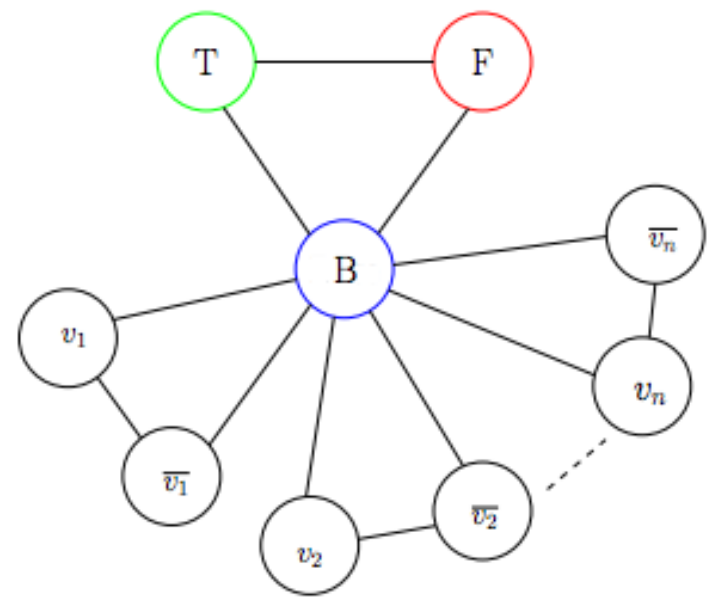
\includegraphics[width=0.5\textwidth]{assets/3-colTFB.png}
\end{figure}

    \item Para cada cl\'ausula $C_j = (a \vee b \vee c)$, introducir un \textit{OR-gadget} (\textbf{Clause Satisfiability Gadget}) con v\'ertices y conexiones que capturen el valor de $a \vee b \vee c$. El gadget se conecta a los v\'ertices correspondientes de los literales $a$, $b$, y $c$, y a los v\'ertices $B$ y $F$. Esto permite que si al menos uno de los literales tiene el color \textit{T}, el nodo salida también se colorea como \textit{T}, y solo se coloreará como \textit{F} cuando todos los literales se coloreen como \textit{F}.
\end{enumerate}

\begin{figure}[h]
    \centering
    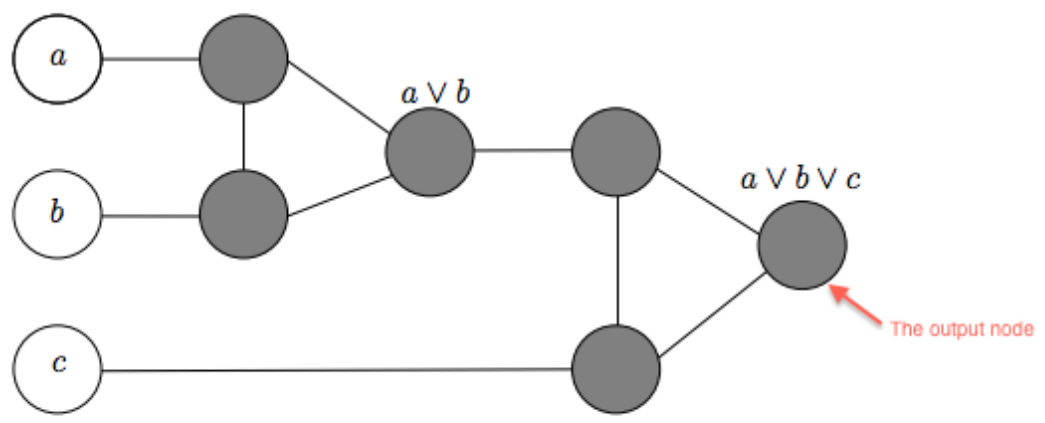
\includegraphics[width=0.7\textwidth]{assets/3-colOR-gadget.png}
\end{figure}

\newpage

Finalmente, el vértice de salida de cada gadget se conecta a los vértices \textit{B} y \textit{F} del triángulo inicial, lo
que asegura que solo pueda ser coloreado como \textit{T} .

\begin{figure}[h]
    \centering
    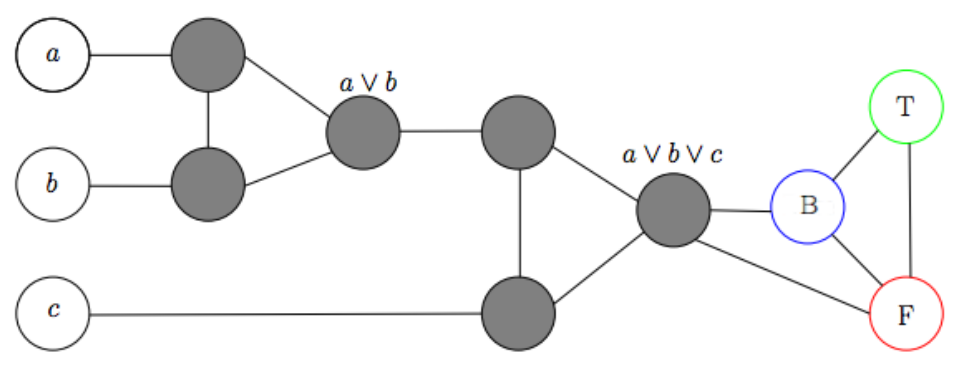
\includegraphics[width=0.8\textwidth]{assets/3-colTFBOR.png}
\end{figure}

\textbf{Probemos que: Si $F$ es satisfacible, entonces $G$ es 3-colorable.}\\
Sea $t$ una asignaci\'on de verdad que satisface $F$. Asignamos colores a los v\'ertices de $G$ como sigue:
\begin{itemize}
    \item Si una variable $x_i$ es verdadera en $t$, coloreamos el v\'ertice $x_i$ con el color $T$ y el v\'ertice $\neg x_i$ con el color $F$.
    \item Para cada cl\'ausula $C_j$, al menos uno de los literales en $C_j$ es verdadero. Usamos el \textit{OR-gadget} para colorear los v\'ertices de manera que el nodo de salida reciba el color $T$, reflejando la satisfacibilidad de la cl\'ausula.
\end{itemize}
Esto asegura que no haya dos v\'ertices adyacentes con el mismo color.

\textbf{Probemos que: Si $G$ es 3-colorable, entonces $F$ es satisfacible.}\\
Dada una coloraci\'on v\'alida de $G$, asignamos valores de verdad a las variables de $F$ como sigue:
\begin{itemize}
    \item Si el v\'ertice $x_i$ tiene el color $T$, asignamos \textit{True} a $x_i$. Si el v\'ertice $\neg x_i$ tiene el color $T$, asignamos \textit{False} a $x_i$.
    \item Para cada cl\'ausula $C_j$, al menos uno de los v\'ertices correspondientes a sus literales debe tener el color $T$, garantizando que la cl\'ausula est\'e satisfecha.
\end{itemize}
Por lo tanto, $t$ satisface $F$.

\subsubsection{Conclusi\'on:} Como la construcci\'on de $G$ se realiza en tiempo polinomial y la satisfacibilidad de $F$ es equivalente a la colorabilidad de $G$, \textbf{3-Coloreo} es NP-Hard.

\subsection{NP-Completitud}
Dado que \textbf{3-Coloreo} pertenece a NP y es NP-Hard, concluimos que es NP-Completo.




\section{N\'umero Crom\'atico}

El problema del \textbf{N\'umero Crom\'atico} se define como sigue:

\textbf{Definici\'on:} El n\'umero crom\'atico de un grafo $G = (V, E)$ es el n\'umero m\'inimo de colores necesarios para colorear los v\'ertices del grafo de manera que dos v\'ertices adyacentes no compartan el mismo color.

\textbf{Problema:} Determinar el n\'umero crom\'atico de un grafo $G$.

\subsection{Pertenencia a NP}

A diferencia de los problemas de decisi\'on como \textbf{3-Coloreo}, no se conoce un algoritmo polinomial para determinar el n\'umero crom\'atico de un grafo, por lo que no podemos asegurar su pertenencia o no a la clase NP.


\subsection{NP-Hardness}

Sin embargo, podemos demostrar que determinar el n\'umero crom\'atico es \textbf{NP-Hard} al reducir polinomialmente desde un problema NP-Completo como \textbf{3-Coloreo}.


\subsubsection{Demostración. Reducci\'on desde 3-Coloreo}
El problema \textbf{3-Coloreo} es un caso especial del problema del n\'umero crom\'atico, donde se pregunta si el n\'umero crom\'atico de un grafo es a lo sumo 3. Aprovecharemos esta relaci\'on para construir la reducci\'on.

Para ello debemos convertir una entrada de \textbf{3-Coloreo} en una entrada de \textbf{Número Cromático} en tiempo polinomial y resolver \textbf{3-Coloreo} a partir de la salida de \textbf{Número Cromático}, también en tiempo polinomial. La entrada de \textbf{3-Coloreo} es un grafo $G = (V, E)$, que será la misma entrada de \textbf{Número Cromático}. Luego, al resolver \textbf{Número Cromático} obtenemos la cantidad mínima de colores necesarios para colorear el grafo sin que dos nodos adyacentes tengan el mismo color. Convertiremos esa salida en una solución para \textbf{3-Coloreo} de la siguiente forma:
\begin{itemize}
    \item Si la cantida de colores es menor o igual a 3 $\Rightarrow$ \textbf{3-Coloreo} es \textit{True}.
    \item Si la cantidad de colores es mayor que 3 $\Rightarrow$ \textbf{3-Coloreo} es \textit{False}.
\end{itemize}

Por lo tanto, resolver el problema del \textbf{N\'umero crom\'atico} en $G$ nos permite decidir si $G$ es 3-colorable, completando la reducci\'on.

\subsubsection{Conclusi\'on}
Como el problema \textbf{3-Coloreo} es NP-Completo, y hemos demostrado que puede reducirse polinomialmente al problema del \textbf{N\'umero crom\'atico}, concluimos que determinar el n\'umero crom\'atico es \textbf{NP-Hard}.

\subsection{NP-Completitud}

Dado que no se conoce si el problema del \textbf{N\'umero crom\'atico} pertenece a NP, tampoco se puede afirmar que sea NP-Completo.




\section{Clique M\'aximo}


\textbf{Definici\'on:} Un clique es un subgrafo completo dentro de un grafo. Formalmente, un clique en un grafo $G = (V, E)$ es un subconjunto de v\'ertices $C \subseteq V$, tal que todos los pares de v\'ertices en $C$ est\'an conectados directamente por una arista. En otras palabras, todos los v\'ertices del clique est\'an mutuamente conectados.

\textbf{Problema:} Determinar el clique de mayor tama\~no en un grafo $G$.

\subsection{Pertenencia a NP}
A diferencia de los problemas de decisi\'on como \textbf{k-Clique}, no se conoce un algoritmo polinomial para determinar el clique de mayor tama\~no en un grafo, por lo que no podemos asegurar su pertenencia o no a la clase NP.

\subsection{NP-Hardness}

Sin embargo, podemos demostrar que determinar el clique m\'aximo es \textbf{NP-Hard} al reducir polinomialmente desde un problema NP-Completo como \textbf{k-Clique}.

\subsubsection{Demostraci\'on. Reducci\'on desde k-Clique}
El problema \textbf{k-Clique} es un caso especial del problema del clique m\'aximo, donde se pregunta si existe un clique de tama\~no exactamente $k$. Aprovecharemos esta relaci\'on para construir la reducci\'on.

Para ello debemos convertir una entrada de \textbf{k-Clique} en una entrada de \textbf{Clique M\'aximo} en tiempo polinomial y resolver \textbf{k-Clique} a partir de la salida de \textbf{Clique M\'aximo}, tambi\'en en tiempo polinomial. La entrada de \textbf{k-Clique} es un grafo $G = (V, E)$ y un entero $k$. La entrada para \textbf{Clique M\'aximo} será el mismo grafo $G = (V, E)$. Luego, al resolver \textbf{Clique M\'aximo} obtenemos el clique m\'aximo y su tamaño en $G$. Convertiremos esa salida en una soluci\'on para \textbf{k-Clique} de la siguiente forma:
\begin{itemize}
    \item Si el tama\~no del clique m\'aximo es mayor o igual a $k$ $\Rightarrow$ \textbf{k-Clique} es \textit{True}.
    \item Si el tama\~no del clique m\'aximo es menor que $k$ $\Rightarrow$ \textbf{k-Clique} es \textit{False}.
\end{itemize}

Por lo tanto, resolver el problema del \textbf{Clique M\'aximo} en $G$ nos permite decidir si $G$ tiene un clique de tama\~no $k$, completando la reducci\'on.

\subsubsection{Conclusi\'on}
Como el problema \textbf{k-Clique} es NP-Completo, y hemos demostrado que puede reducirse polinomialmente al problema del \textbf{Clique M\'aximo}, concluimos que determinar el clique m\'aximo es \textbf{NP-Hard}.

\subsection{NP-Completitud}

Dado que no se conoce si el problema del \textbf{Clique M\'aximo} pertenece a NP, tampoco se puede afirmar que sea NP-Completo.



\section{Cobertura de Cliques}


\textbf{Definici\'on:} Dado un grafo $G = (V, E)$, una cobertura de cliques es un conjunto de cliques $C_1, C_2, \dots, C_k$ tal que cada arista $(u, v) \in E$ pertenece a al menos uno de estos cliques.

\textbf{Problema:} Determinar el n\'umero m\'inimo de cliques necesarios para cubrir todas las aristas del grafo.

\subsection{Pertenencia a NP}

El problema de \textbf{Cobertura de Cliques} pertenece a NP, ya que, dado un conjunto de cliques, es posible verificar en tiempo polinomial si cada arista en E está cubierta por
al menos uno de los cliques. 



\subsection{NP-Hardness}

Podemos demostrar que \textbf{Cobertura de Cliques} es NP-Hard al reducir polinomialmente desde un problema NP-Completo como \textbf{N\'umero Crom\'atico}.

\subsubsection{Demostraci\'on. Reducci\'on desde N\'umero Crom\'atico}
El problema \textbf{N\'umero Crom\'atico} pregunta por el n\'umero m\'inimo de colores necesarios para colorear los v\'ertices de un grafo de modo que no haya dos v\'ertices adyacentes con el mismo color. 
Se conoce que un conjunto de vértices en un grafo $G$ es un clique si y solo si es un conjunto independiente en el grafo complemento $G^c$. Una partición de los vértices de $G$ en cliques
(cobertura de cliques de $G$) corresponde a una partición de $G^c$ en conjuntos independientes. Una coloración de un grafo es un partición de sus vértices en conjuntos independientes. Por lo tanto, una cobertura de cliques de $G$ 
será una coloración de $G^c$, por lo que la cobertura mínima de $G$ será el número cromático de $G^c$.

Aprovecharemos esta relaci\'on para construir la reducci\'on. La entrada de \textbf{N\'umero Crom\'atico} es un grafo $G = (V, E)$.



\paragraph{Construcci\'on:} Dado un grafo $G = (V, E)$, construimos un grafo complementario $G^c = (V, E^c)$, donde $E^c$ contiene todas las aristas que no est\'an en $E$. La entrada para \textbf{Cobertura de Cliques} ser\'a $G^c$.
Luego de resolver \textbf{Cobertura de Clique} en $G^c$ obtendremos un $k$ que es la mínima cantidad de cliques en que podemos particionar el grafo tal que cada arista esté contenida en al menos uno de esos cliques, que es equivalente a la cantidad de conjuntos independientes de $G$, que a su vez es equivalente a su número cromático.


Por lo tanto, resolver el problema de \textbf{Cobertura de Cliques} en $G^c$ nos permite decidir el n\'umero crom\'atico de $G$, completando la reducci\'on.

\subsubsection{Conclusi\'on}
Como el problema \textbf{N\'umero Crom\'atico} es NP-Completo, y hemos demostrado que puede reducirse polinomialmente al problema de \textbf{Cobertura de Cliques}, concluimos que \textbf{Cobertura de Cliques} es \textbf{NP-Hard}.

\subsection{NP-Completitud}

Como \textbf{Cobertura de Cliques} es \textbf{NP} y \textbf{NP-Hard}, podemos concluir que es \textbf{NP-Completo}.



\section{Conjunto Dominante}


\textbf{Definici\'on:} En un grafo $G = (V, E)$, un conjunto de v\'ertices $D \subseteq V$ es un conjunto dominante si cada v\'ertice de $V$ que no est\'a en $D$ es adyacente a al menos un v\'ertice en $D$. 

\textbf{Problema:} Determinar el conjunto dominante de menor cardinalidad en un grafo $G$. 

\subsection{Pertenencia a NP}

El problema \textbf{Conjunto Dominante} pertenece a NP porque, dado un conjunto candidato $D$, podemos verificar en tiempo polinomial si $D$ domina todos los v\'ertices de $G$. 

\subsection{NP-Hardness}
Podemos demostrar que \textbf{Conjunto Dominante} es NP-Hard mediante una reducci\'on desde el problema \textbf{Vertex Cover}, que se conoce que es NP-Completo.

\subsubsection{Demostraci\'on. Reducci\'on desde Vertex Cover}
Dado un grafo $G = (V, E)$ como entrada para el problema \textbf{Vertex Cover}, construiremos un grafo $G' = (V', E')$ tal que:
\begin{itemize}
    \item $V'$ contiene todos los v\'ertices de $V$ y, por cada arista $(u, v) \in E$, un nuevo v\'ertice $w$.
    \item $E'$ incluye todas las aristas de $E$ m\'as dos nuevas aristas $(u, w)$ y $(w, v)$ para cada arista $(u, v)$ de $E$.
\end{itemize}

La construcci\'on de $G'$ se realiza en tiempo polinomial, ya que solo duplicamos las aristas y agregamos un nuevo v\'ertice por cada arista original.

\textbf{Probemos que: Si $S$ es un vertex cover en $G$, entonces $S$ tambi\'en es un conjunto dominante en $G'$.}\\
    Como $S$ es un vertex cover, cada arista en $G$ tiene al menos un extremo en $S$. Consideremos $v \in G'$. Si $v$ es un nodo original de $G$, entonces
    o $v \in S$ o debe existir alguna arista que conecte a $v$ a otro nodo $u$. Como $S$ es un vertex cover, si $v \notin S$, entonces $u$ tiene que estar en $S$, por lo que habría un nodo adyacente a $v$ en $S$. Entonces $v$ está cubierto por algún elemento de $S$.
    Por otra parte, si $w$ es un nodo adicional en $G'$ entonces tiene dos nodos adyacentes $u$ y $v \in G$ y utilizando el argumento anterior al menos uno de ellos está en $S$.
    Entonces los nodos adicionales también están cubiertos por $S$. Entonces si $G$ tiene un vertex cover, $G'$ tendrá un conjunto dominante de al menos el mismo tamaño.
    

\textbf{Probemos que: Si $D$ es un conjunto dominante de tamaño $k$ de $G$, entonces en $G'$ existe eun vertex cover de tamaño a lo sumo $k$.} \\
Si $D$ es un conjunto dominante de tamaño $k$ en $G'$, consideremos todos los vértices adicionales $w \in D$. 
Observemos que $w$ debe estar conectado exactamente a dos vértices $u,v \in G$.
Ahora, podemos reemplazar $w$ de manera segura por $u$ o $v$. El vértice $w$ en $D$ nos ayudará a dominar solo a $u, v, w \in G'$.
Sin embargo, estas tres aristas forman un ciclo de 3 (\textit{3-cycle}), por lo que podemos elegir $u$ o $v$ y seguir dominando todos los vértices que $w$ dominaba anteriormente. 
De esta manera, podemos eliminar todos los vértices adicionales de la forma descrita. 
Dado que todos los vértices adicionales corresponden a una de las aristas en $G$, y dado que todos los vértices adicionales están cubiertos por el conjunto $D$ modificado, esto significa que todas las aristas en $G$ están cubiertas por el conjunto.
Por lo tanto, si $G'$ tiene un conjunto dominante de tamaño $k$, entonces $G$ tiene un vertex cover de tamaño a lo sumo $k$.



Así, hemos probado ambos lados de la equivalencia. Existe un conjunto dominante de tamaño $k$ en $G'$ si y solo si existe un vertex cover de tamaño $k$ en $G$. 

\subsubsection{Conclusión}
Dado que sabemos que el problema \textbf{Vertex Cover} es NP-Completo, y demostramos que es posible hacer una reducción en tiempo polinomial de \textbf{Vertex Cover} a \textbf{Conjunto Dominante}, el problema \textbf{Conjunto Dominante} es NP-Hard.


\subsection{NP-Completitud}

Como \textbf{Conjunto Dominante} es NP-Hard y pertenece a NP, concluimos que es NP-Completo.


\section{Retroalimentaci\'on de V\'ertices}


\textbf{Definici\'on:} Dado un grafo $G = (V, E)$, un conjunto de retroalimentaci\'on de v\'ertices es un subconjunto de v\'ertices $F \subseteq V$ tal que al eliminar todos los v\'ertices en $F$ (y sus aristas incidentes), el grafo resultante no contiene ciclos (es decir, el grafo resultante es ac\'iclico o un bosque, si es no dirigido).

\textbf{Problema:} Encontrar el conjunto de retroalimentaci\'on de v\'ertices de tama\~no m\'inimo.

\subsection{Pertenencia a NP}
El problema \textbf{Retroalimentaci\'on de V\'ertices} pertenece a NP porque, dado un conjunto candidato $F$, podemos verificar en tiempo polinomial si eliminar $F$ hace que el grafo sea ac\'iclico. 

\subsection{NP-Hardness}
Podemos demostrar que \textbf{Retroalimentaci\'on de V\'ertices} es NP-Hard mediante una reducci\'on desde el problema \textbf{Vertex Cover}, que es conocido como NP-Completo.

\subsubsection{Demostraci\'on. Reducci\'on desde Vertex Cover}
Dado un grafo no dirigido $G = (V, E)$ y un entero $k$ como entrada para el problema \textbf{Vertex Cover}, construiremos un grafo $G' = (V', E')$ como sigue:
\begin{itemize}
    \item Por cada v\'ertice $v \in V$, incluimos un v\'ertice correspondiente $v \in V'$.
    \item Por cada arista $e = (u, v) \in E$, agregamos un nuevo v\'ertice $w$ en $V'$.
    \item En $E'$, incluimos las aristas $(u, v)$, $(u, w)$, y $(w, v)$ para cada arista $e = (u, v)$ en $E$.
\end{itemize}

Esta construcci\'on de $G'$ se realiza en tiempo polinomial, ya que simplemente agregamos un nuevo v\'ertice y dos nuevas aristas por cada arista en $G$.

\begin{itemize}
    \item \textbf{Probemos que: Si $S$ es un vertex cover en $G$ de tama\~no $k$, entonces $S$ tambi\'en es un conjunto de retroalimentaci\'on de v\'ertices en $G'$ de tama\~no $k$.}\\
    Como $S$ es un vertex cover, cada arista $(u, v)$ en $G$ tiene al menos un extremo en $S$. En $G'$, cualquier ciclo debe incluir una de las aristas $(u, v)$, $(u, w)$ o $(w, v)$. Dado que $S$ contiene al menos uno de los extremos de $(u, v)$, cualquier ciclo en $G'$ intersecta con $S$. Por lo tanto, eliminar $S$ asegura que $G'$ sea ac\'iclico.

    \item \textbf{Probemos que: Si $F$ es un conjunto de retroalimentaci\'on de v\'ertices en $G'$ de tama\~no $k$, entonces $F$ contiene un conjunto equivalente en $G$ que es un vertex cover.}\\
    Consideremos cualquier ciclo en $G'$. Dicho ciclo debe incluir uno de los v\'ertices adicionales $w$ correspondientes a una arista $(u, v)$ en $G$. En este caso, podemos reemplazar $w$ por uno de sus extremos $u$ o $v$ en $F$, ya que eliminar $u$ o $v$ es suficiente para romper todos los ciclos que incluyen $w$. Finalmente, dado que todos los ciclos en $G'$ se corresponden con las aristas de $G$, $F$ debe contener un v\'ertice de cada arista en $G$, lo que implica que $F$ es un vertex cover en $G$.
\end{itemize}


\subsubsection{Conclusión}
Dado que $S$ es un vertex cover de tama\~no $k$ en $G$ si y solo si $F$ es un conjunto de retroalimentaci\'on de v\'ertices de tama\~no $k$ en $G'$, y como sabemos que \textbf{Vertex Cover} es NP-Completo, hemos probado que \textbf{Retroalimentaci\'on de V\'ertices} es NP-Hard.

\subsection{NP-Completitud}

Como \textbf{Retroalimentaci\'on de V\'ertices} es NP-Hard y pertenece a NP, concluimos que es NP-Completo.




\section{Retroalimentaci\'on de Arcos}

\textbf{Definici\'on:} Dado un grafo dirigido $G = (V, E)$, un conjunto de retroalimentaci\'on de arcos es un subconjunto de arcos $F \subseteq E$ tal que, al eliminar todos los arcos en $F$, el grafo resultante no contiene ciclos (es decir, el grafo resultante es ac\'iclico).

\textbf{Problema:} Encontrar el conjunto de retroalimentaci\'on de arcos de tama\~no m\'inimo.

\subsection{Pertenencia a NP}
El problema \textbf{Retroalimentaci\'on de Arcos} pertenece a NP porque, dado un conjunto candidato $F$, podemos verificar en tiempo polinomial si eliminar $F$ hace que el grafo sea ac\'iclico. 
\subsection{NP-Hardness}
Podemos demostrar que \textbf{Retroalimentaci\'on de Arcos} es NP-Hard mediante una reducci\'on desde el problema \textbf{Retroalimentaci\'on de V\'ertices}, que demostramos que es NP-Completo.

\subsubsection{Demostraci\'on. Reducci\'on desde Retroalimentaci\'on de V\'ertices}
Dado un grafo $G = (V, E)$ y un entero $k$ como instancia del problema \textbf{Retroalimentaci\'on de V\'ertices}, construiremos una instancia $(G', k')$ del problema \textbf{Retroalimentaci\'on de Arcos} como sigue:
\begin{itemize}
    \item Por cada v\'ertice $v \in V$, creamos dos nuevos v\'ertices $v_1$ y $v_2$ en $G'$ y a\~nadimos el arco interno $(v_1, v_2)$.
    \item Por cada arco $(u, v) \in E$ en el grafo original, a\~nadimos un arco externo $(u_2, v_1)$ en $G'$.
\end{itemize}

Gracias a esto, cada v\'ertice en $G$ se duplica en $G'$. Los arcos del grafo original se dividen en:
\begin{itemize}
    \item \textbf{Arcos internos:} Entre las dos copias de un mismo v\'ertice, $(v_1, v_2)$.
    \item \textbf{Arcos externos:} Entre las copias de v\'ertices diferentes, $(u_2, v_1)$.
\end{itemize}

Resolver \textbf{Retroalimentaci\'on de Arcos} en $G'$ equivale a encontrar un conjunto de arcos cuyo borrado elimine todos los ciclos en $G'$. 
Nótese que cualquier ciclo que contenga arcos externos tambi\'en debe pasar por al menos un arco interno $\Rightarrow$ eliminar s\'olo arcos internos (que corresponden a eliminar v\'ertices en $G$) es suficiente para romper los ciclos.

\paragraph{Correctitud:}
\begin{itemize}
    \item Cualquier conjunto de arcos internos que forme una soluci\'on para \textbf{Retroalimentaci\'on de Arcos} en $G'$ corresponde a un conjunto de v\'ertices que forman una soluci\'on para \textbf{Retroalimentaci\'on de V\'ertices} en $G$.\\
    Esto se debe a que romper los ciclos en $G'$ eliminando arcos internos es equivalente a romper los ciclos en $G$ eliminando los v\'ertices correspondientes.
    \item Por otro lado, cualquier conjunto de v\'ertices en $G$ que rompa todos los ciclos se puede traducir directamente a un conjunto de arcos internos en $G'$ que rompa los ciclos en $G'$.
\end{itemize}

Por lo tanto, resolver \textbf{Retroalimentaci\'on de Arcos} en $G'$ es equivalente a resolver \textbf{Retroalimentaci\'on de V\'ertices} en $G$.

\subsubsection{Conclusi\'on}
Dado que \textbf{Retroalimentaci\'on de V\'ertices} es NP-Completo, y hemos demostrado que se puede reducir polinomialmente al problema \textbf{Retroalimentaci\'on de Arcos}, concluimos que \textbf{Retroalimentaci\'on de Arcos} es NP-Hard.

\subsection{NP-Completitud}

Como \textbf{Retroalimentaci\'on de Arcos} es NP-Hard y pertenece a NP, concluimos que es NP-Completo.



\section{NAE 4-SAT (Not-All-Equal 4-SAT)}

\textbf{Definici\'on:} Dada una f\'ormula booleana en CNF donde cada cl\'ausula tiene exactamente 4 literales, determinar si existe una asignaci\'on de valores de verdad a las variables de modo que en cada cl\'ausula no todos los literales sean verdaderos ni todos sean falsos.

\subsection{Pertenencia a NP}
El problema \textbf{NAE 4-SAT} pertenece a NP porque, dada una asignaci\'on de valores de verdad a las variables, podemos verificar en tiempo polinomial si no todos los literales en cada cl\'ausula son iguales y la fórmula es satisfacible.

\subsection{NP-Hardness}

Demostraremos que \textbf{NAE 4-SAT} es NP-Hard mediante una reducci\'on desde \textbf{3-SAT}.

\subsubsection{Demostraci\'on. Reducción desde 3-SAT}
Dada una instancia de \textbf{3-SAT} $\phi$, construiremos una instancia equivalente de \textbf{NAE 4-SAT} $\phi'$ en tiempo polinomial. Para ello agregamos una nueva variable $z$ a cada cl\'ausula de $\phi$.
Demostremos que $\phi$ es satisfacible si y solo si $\phi'$ es satisfacible. \\

$(\Rightarrow)$ Si $x_1, \ldots, x_n$ es una asignación satisfacible para $\phi$, entonces la misma asignación satisface $\phi'$ cuando elegimos $z=0$. \\

$(\Leftarrow)$ Supongamos que $x_1, \ldots, x_n, z$ es una asignación satisfacible de $\phi'$. Nótese que
$\neg{x_1}, \ldots, \neg{x_n}, \neg{z}$ también es una asignación satisfacible de $\phi'$ (porque $NAE(a,b,c,d) = NAE(\neg{a},\neg{b},\neg{c},\neg{d})$).
En una de estas dos asignaciones, el valor asignado a $z$ es 0. Esa asignación corresponde a una asignación satisfacible para $\phi$.\\



\subsubsection{Conclusi\'on}
Como \textbf{3-SAT} es NP-Completo, y hemos demostrado una reducci\'on polinomial hacia \textbf{NAE 4-SAT}, concluimos que \textbf{NAE 4-SAT} es NP-Hard. 

\subsection{NP-Completitud}

Como \textbf{NAE 4-SAT} pertenece a NP y es NP-Hard, es NP-Completo.

\section{NAE 3-SAT (Not-All-Equal 3-SAT)}

\textbf{Definici\'on:} Dada una f\'ormula booleana en CNF donde cada cl\'ausula tiene exactamente 3 literales, determinar si existe una asignaci\'on de valores de verdad a las variables de modo que en cada cl\'ausula no todos los literales sean verdaderos ni todos sean falsos.

\subsection{Pertenencia a NP}
El problema \textbf{NAE 3-SAT} pertenece a NP porque, dada una asignaci\'on de valores de verdad a las variables, podemos verificar en tiempo polinomial si no todos los literales en cada cl\'ausula son iguales y la fórmula sea satisfacible.

\subsection{NP-Hardness}

Demostraremos que \textbf{NAE 3-SAT} es NP-Hard mediante una reducci\'on desde \textbf{NAE 4-SAT}.

\subsubsection{Demostraci\'on. Reducción desde NAE 4-SAT}
Dada una instancia de \textbf{NAE 4-SAT} $\phi$, construiremos una instancia equivalente de \textbf{NAE 3-SAT} $\phi'$ en tiempo polinomial. Para cada cl\'ausula $\text{NAE}(a, b, c, d)$ en $\phi$:
\begin{itemize}
    \item Introducimos una nueva variable $w$.
    \item Reemplazamos $\text{NAE}(a, b, c, d)$ por las cl\'ausulas $\text{NAE}(a, b, w)$ y $\text{NAE}(\neg w, c, d)$ en $\phi'$.
\end{itemize}

La demostración se basa en que cuatro valores booleanos $a, b, c, d$ no son todos iguales si y solo si existe un valor $w$ tal que $\text{NAE}(a, b, w)$ y $\text{NAE}(\neg w, c, d)$ son verdaderos.

\subsubsection{Conclusi\'on}
Como \textbf{NAE 4-SAT} es NP-Completo, y hemos demostrado una reducci\'on polinomial hacia \textbf{NAE 3-SAT}, concluimos que \textbf{NAE 3-SAT} es NP-Hard. 

\subsection{NP-Completitud}
Como \textbf{NAE 3-SAT} pertenece a NP y es NP-Hard, es NP-Completo.

\section{Máximo Corte}

\textbf{Definici\'on:} Sea $G = (V, E)$ un grafo con aristas ponderadas. Un corte es una divisi\'on de los v\'ertices en dos conjuntos $T$ y $V - T$. El costo de un corte es la suma de los pesos de las aristas que van de $T$ a $V - T$. El problema \textbf{Máximo Corte} consiste en determinar si existe un corte con costo al menos $c$ en un grafo dado.

\subsection{Pertenencia a NP}

El problema \textbf{Máximo Corte} pertenece a NP porque, dado un corte $T$, podemos verificar en tiempo polinomial si su costo es al menos $c$ sumando los pesos de las aristas de cruce del corte.

\subsection{NP-Hardness}

Demostraremos que \textbf{Máximo Corte} es NP-Hard mediante una reducci\'on desde \textbf{NAE 3-SAT}.

\subsubsection{Demostraci\'on. Reducción desde NAE 3-SAT}
Dada una instancia de \textbf{NAE 3-SAT} $\phi$, construiremos una instancia equivalente de \textbf{Máximo Corte} $(G, c)$ como sigue:
\begin{itemize}
    \item Por cada variable $x_i$ de $\phi$, agregamos dos v\'ertices en $G$ etiquetados como $x_i$ y $\neg x_i$, conectados por una arista con capacidad $M = 10 \cdot m$, donde $m$ es el n\'umero de cl\'ausulas en $\phi$.
    \item Por cada cl\'ausula $C$ en $\phi$, agregamos un tri\'angulo entre los v\'ertices correspondientes a los t\'erminos en $C$, con aristas de capacidad 1.
\end{itemize}

Demostremos que $G$ contiene un corte con capacidad al menos $nM+2m$ (donde $n$ es el número de variables) si y solo si $\phi$ es satisfacible.
\begin{itemize}
    \item $(\Leftarrow)$ Si $\phi$ es satisfactible, entonces existe un corte en $G$ con capacidad al menos $nM + 2m$:
    Supongamos que $\phi$ es satisfacible y consideremos cualquier asignación satisfacible. Esta asignación corresponde a un corte en $G$ (Un lado del corte consiste en todos los vértices etiquetados por términos que evalúan 1 en la asignación. El otro lado consiste en todos los vértices etiquetados por términos que evalúan 0). 
    Este corte tiene capacidad el menos $nM+2m$ porque:
    \begin{itemize}
        \item Como exactamente uno de los términos $x_i$ y $\neg{x_i}$ evalúa 1 en la asignación, todos los arcos entre $x_i$ y $\neg x_i$ cruzan el corte (contribuyendo $n \cdot M$).
        \item Como la asignación satisface $\phi$, exactamente dos aristas en cada tri\'angulo cruzan el corte (contribuyendo $2 \cdot m$).
    \end{itemize}
    \item $(\Rightarrow)$ Si existe un corte con capacidad al menos $n \cdot M + 2 \cdot m$, entonces corresponde a una asignaci\'on satisfactoria para $\phi$:
    Supongamos que $G$ contiene un corte con capacidad el menos $nM+2m$. Probemos que:
    \begin{itemize}
        \item Todas las aristas entre $x_i$ y $\neg x_i$ cruzan el corte, garantizando una asignaci\'on consistente. Esto ocurre
        porque cualquier corte que no contenga una de estas aristas tendrá como mucho capacidad $(n-1)M+3m=nM+3m-10m$, que es estrictamente menor que $nM+2m$.
        \item Exactamente dos aristas en cada tri\'angulo cruzan el corte, satisfaciendo cada cl\'ausula de $\phi$. Esto ocurre porque ningún corte puede separar las tres aristas de un triángulo y
        por lo tanto si un corte separa menos de dos aristas en uno de los triángulos de cláusula, entonces su capacidad es estrictamente menor que $nM+2m$. 

    \end{itemize}
Como todas las aristas entre $x_i$ y $\neg x_i$ cruzan el corte, este corresponde a una asignación para $\phi$. 
Además, como exactamente dos aristas en cada tri\'angulo cruzan el corte, la asignaci\'on correspondiente es satisfactible.
\end{itemize}

\subsubsection{Conclusi\'on}
Como \textbf{NAE 3-SAT} es NP-Completo, y hemos demostrado una reducci\'on polinomial hacia \textbf{Máximo Corte}, concluimos que \textbf{Máximo Corte} es NP-Hard. 

\subsection{NP-Completitud}

Como \textbf{Máximo Corte} pertenece a NP y es NP-Completo, es NP-Completo.

\end{document}